\newpage

\section{VPN}
\opnsense\ has two different VPN solutions built-in. It is IPsec and OpenVPN. There is also possible to use L2TP (Legacy), PPTP (Legacy), OpenConnect, Stunnel, Tinc, WireGuard, and ZeroTier via installing plugins. This tutorial will use OpenVPN.

Two different connection methods could be used when using VPN. Site to site and client-server tunnel. Site to site is used to connect two or more different sites. For example, a business that has multiple divisions that need to connect back to a headquarter. A client-server tunnel is when someone is connecting to the business network remotely. In this tutorial, the client-server tunnel method is explored.

In this section, you will learn:
\begin{itemize}
    \item How to configure OpenVPN using a client-server tunnel.
    \item Create a CA (Certificate Authority).
    \item Create a new user.
\end{itemize}


\subsection{OpenVPN wizard} % change the title here!
In this task, you are using the VPN wizard to configure the server-side of the VPN service. The wizard will guide you through the steps:

\begin{enumerate}
    \item Create a certificate authority.
    \item Create a certificate.
    \item Configure the VPN server.
    \item Create Firewall rules.
\end{enumerate}

\setupblock{\begin{enumerate}
    \item Goto \cmd{VPN --> OpenVPN --> Servers}.
    \item Click on the button \cmd{Use a wizard to setup a new server}.
    \item Choose \cmd{Local User Access}.
    \item Click on \cmd{Add New CA}.
    \item Configure the following fields:
    \begin{enumerate}
        \item Set \cmd{Descriptive name} to \cmd{opensense\_vpn}.
        \item Set \cmd{Country Code} to \cmd{NO}.
        \item Set \cmd{State or Province} to \cmd{Agder}.
        \item Set \cmd{City} to \cmd{Kristiansand}.
        \item Set \cmd{Organization} to \cmd{Noroff}.
        \item Set \cmd{Email} to the email you use.
    \end{enumerate}
    \item The next step in the wizard is to create the certificate. Click on \cmd{Add new CA}.
    \item Configure the following fields:
    \begin{enumerate}
        \item Set \cmd{Descriptive name} to \cmd{opensense\_cert}.
        \item The other field here should be prefilled from the previous fields you changed.
        \item Click \cmd{Create new Certificate}.
    \end{enumerate}
    \item The next step in the wizard is to setup the OpenVPN server. Change only the following fields:
    \begin{enumerate}
        \item Set \cmd{IPv4 Tunnel Network} to \cmd{192.168.50.0/24}. - A new network that the clients are using when they  are connecting using the VPN.
        \item Set \cmd{IPv4 Local Network} to \cmd{192.168.20.0/24}. - Our original local network.
        \item Set \cmd{DNS server 1} to \cmd{8.8.8.8}. - Google DNS server.
        \item Set \cmd{DNS server 2} to \cmd{8.8.4.4}. - Google DNS server.
        \item Click on \cmd{Next}.
    \end{enumerate}
    \item The next step in the wizard is to configure the firewall rules (figure \ref{opnsense:vpn_rules}). Here you will see two options. The first one is to accept traffic from the newly created network to the internet, and the second one is to accept client traffic to the VPN tunnel.
    \item Check both of them and click the \cmd{Next} button.
    \item Click the \cmd{Finish} button to quit the wizard.
\end{enumerate}}

\begin{figure}[h!]
    \centering
    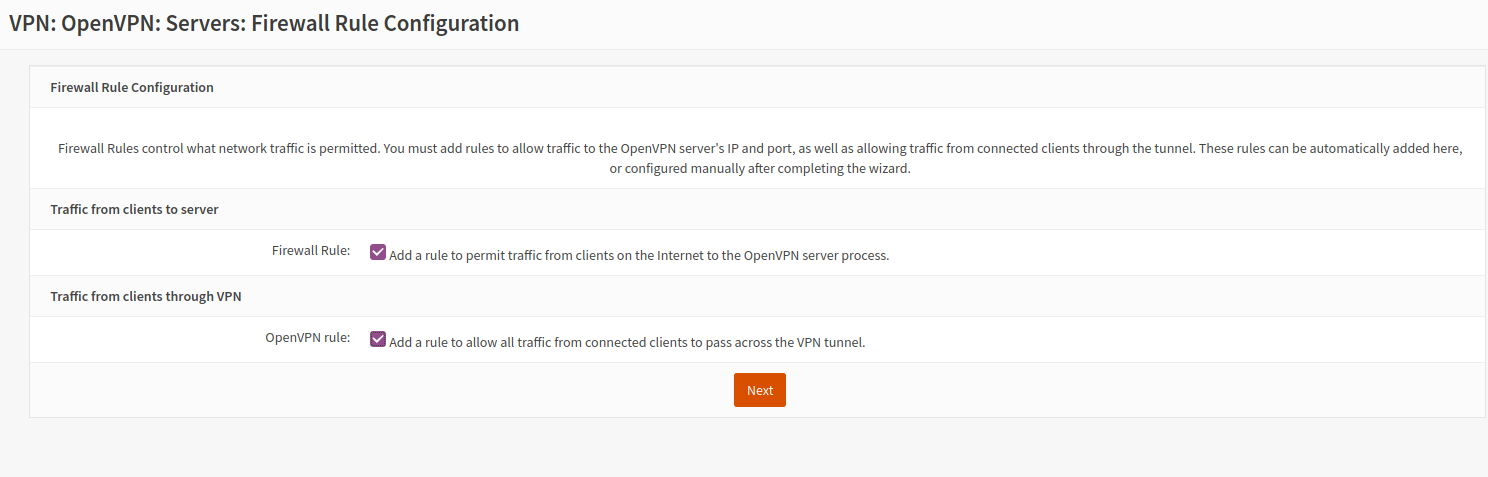
\includegraphics[width=0.9\textwidth]{Images/vpn/firewall_rules.PNG}
    \caption{Adding firewall rules during VPN configuration}
    \label{opnsense:vpn_rules}
\end{figure}

When you are finished with the wizard, the first page after will show you if the VPN service is running (figure \ref{opnsense:vpn_running}). It could also be checked on the \cmd{Dashboard} page.

\begin{figure}[h!]
    \centering
    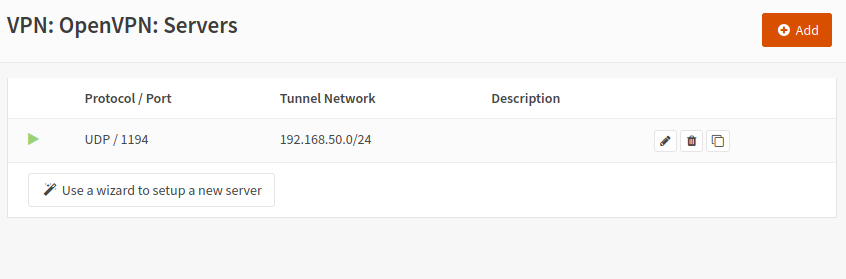
\includegraphics[width=0.9\textwidth]{Images/vpn/vpn.PNG}
    \caption{VPN is running}
    \label{opnsense:vpn_running}
\end{figure}


\subsection{Client setup}
The next step is to create a user with a certificate and get the user to access the VPN network we have created. If you do not have a user, create the user with the guide in \ref{user_groups}. When the user is created, remember to check the box that says \cmd{Certification} and when prompted later for certificate method to use, choose \cmd{Create internal Certificate}.

If you have a user and want to add a certificate to the user:

\setupblock{\begin{enumerate}
    \item Goto \cmd{System --> Access --> Users}.
    \item Locate the user you want to create a certificate for and click on the pencil on the right side of the username.
    \item Click on the plus sign beside \cmd{User Certificate} to add a certificate to an existing user.
    \item Choose \cmd{Create internal Certificate}.
    \item Click \cmd{Save}
\end{enumerate}}

If you go back to the user you either created or modified, there is now a certificate attached to the user (figure \ref{opnsense:vpn_cert_added}).

\begin{figure}[h!]
    \centering
    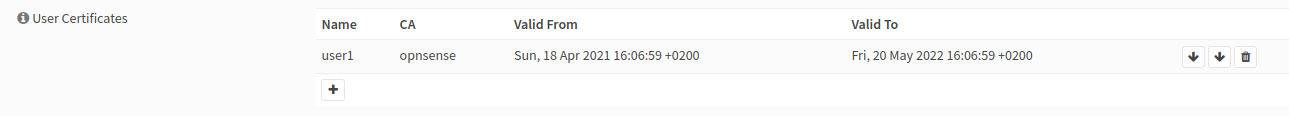
\includegraphics[width=0.9\textwidth]{Images/vpn/user_cert.PNG}
    \caption{Certificate added to user}
    \label{opnsense:vpn_cert_added}
\end{figure}

\subsubsection{Export user certificate and configuration}
To test that the OpenVPN is working correctly, we have two options. We could use the Ubuntu client we are using and connect it to the VPN, this is one simple solution, but not exactly what we want for this solution, since it is not connecting \textbf{remotely}. The second solution is to use our host machine. The following configuration will guide you through the process.

First you need to give the host machine access to the firewalls web interface:

\setupblock{\begin{enumerate}
    \item Goto \cmd{Firewall --> Rules --> Wan}.
    \item Create a new rule using the \cmd{Add} button.
    \item Change this in the configuration:
    \begin{enumerate}
        \item Set \cmd{Protocol} to \cmd{TCP}.
        \item Set \cmd{Destination} to \cmd{This firewall}.
        \item Set \cmd{Destination port range} to \cmd{HTTPS} (on both to and from).
        \item Set \cmd{Description} to \cmd{Access to web interface}.
        \item Optional, make a checkmark in the \cmd{Log} box. - If \cmd{Log} has a checkmark, all packets that are using this rule will be logged. It is recommended since you want to have accounting on who is accessing the web interface.
    \end{enumerate}
    \item Click \cmd{Save} and \cmd{Apply changes}.
\end{enumerate}}

\quesblock{\begin{enumerate}
    \item[34.] Find the \opnsense\ WAN IP address and try to access it from your host. Does it work?
\end{enumerate}}

The next step is to export the certificate and configuration.

\setupblock{\begin{enumerate}
    \item On your host machine, goto \url{https://<YOUR-FIREWALL-WAN-IP-ADRESS>} and login.
    \item Goto \cmd{VPN --> OpenVPN --> Client Export}.
    \item Change this in the configuration:
    \begin{enumerate}
        \item Set \cmd{Hostname} to the WAN IP address your firewall has.
        \item Remove any passwords that are in the configuration.
        \item Remove the checkmark in the \cmd{Validate Server Subject} box.
        \item At the bottom, there is a cloud symbol to the right of the user you want to download the configuration for (see figure \ref{opnsense:vpn_cert_download}).
        \item Download and extract the files on your host. 
    \end{enumerate}
\end{enumerate}}

\begin{figure}[h!]
    \centering
    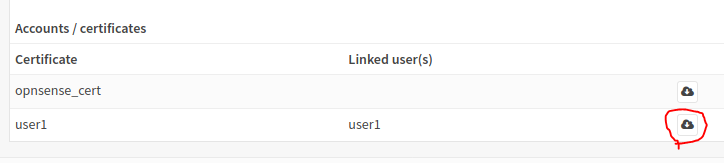
\includegraphics[width=0.7\textwidth]{Images/vpn/user_download_cert.PNG}
    \caption{Download certificate for a user}
    \label{opnsense:vpn_cert_download}
\end{figure}

\subsubsection{Firewall rule for VPN clients}
We need to configure a firewall rule to give VPN clients access to the WAN interface on the firewall. This is the last step on the server-side for the configuration of the OpenVPN server.

\setupblock{\begin{enumerate}
    \item Goto \cmd{Firewall --> Rules --> Wan}.
    \item Create a new rule using the \cmd{Add} button.
    \item Change this in the configuration:
    \begin{enumerate}
        \item Set \cmd{Protocol} to \cmd{UDP}.
        \item Set \cmd{Destination} to \cmd{This firewall}.
        \item Set \cmd{Destination port range} to \cmd{OpenVPN} (on both to and from).
        \item Set a checkmark beside \cmd{Log} to log packets and events.
        \item Set \cmd{Description} to \cmd{Client access to OpenVPN}.
    \end{enumerate}
    \item Click \cmd{Save} and \cmd{Apply changes}.
\end{enumerate}}

\subsubsection{Configure the client}
Start with downloading the OpenVPN client to your host machine. Other options work also, but you are on your own if you decide to do that.

\dlblock{OpenVPN can be downloaded from here, regardless of what OS you have:}{https://openvpn.net/vpn-client/}

\setupblock{\begin{enumerate}
    \item Install the VPN client.
    \item Depending on if you are using a GUI or CLI choose your correct step below.
    \begin{itemize}
        \item GUI: Import the \cmd{.ovnp} file to the VPN client if you are using a GUI version (Goto step \ref{imported}).
        \item CLI: If you are using a CLI version, you can use this command \cmd{sudo openvpn <YOUR OPENVPN FILE HERE>} to connect to the VPN service.
    \end{itemize}
    \item \label{imported} When the file is imported, try to connect and you will be prompt for username and password (figure \ref{opnsense:vpn_openvpn_up}).
\end{enumerate}}

\tipbox{If you have a problem connecting with the GUI version, make sure that all of the files you downloaded is in the correct folder. Check the OpenVPN settings to see where the files are moved when they are imported.}

\begin{figure}[h!]
    \centering
    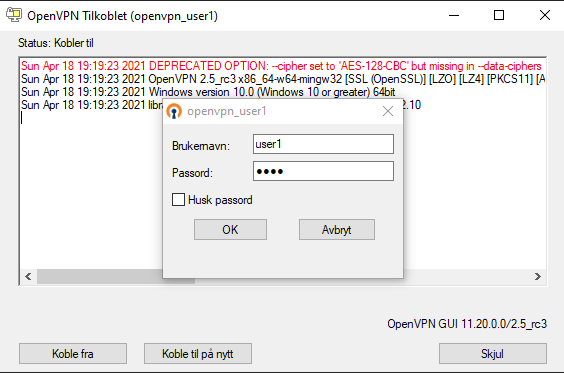
\includegraphics[width=0.5\textwidth]{Images/vpn/vpn_client_connecting.PNG}
    \caption{OpenVPN asks for username and password}
    \label{opnsense:vpn_openvpn_up}
\end{figure}

Goto \cmd{VPN --> OpenVPN --> Connection Status} to see if the client (your host machine) connected to the VPN network we created (figure \ref{opnsense:vpn_openvpn_status}).

\begin{figure}[h!]
    \centering
    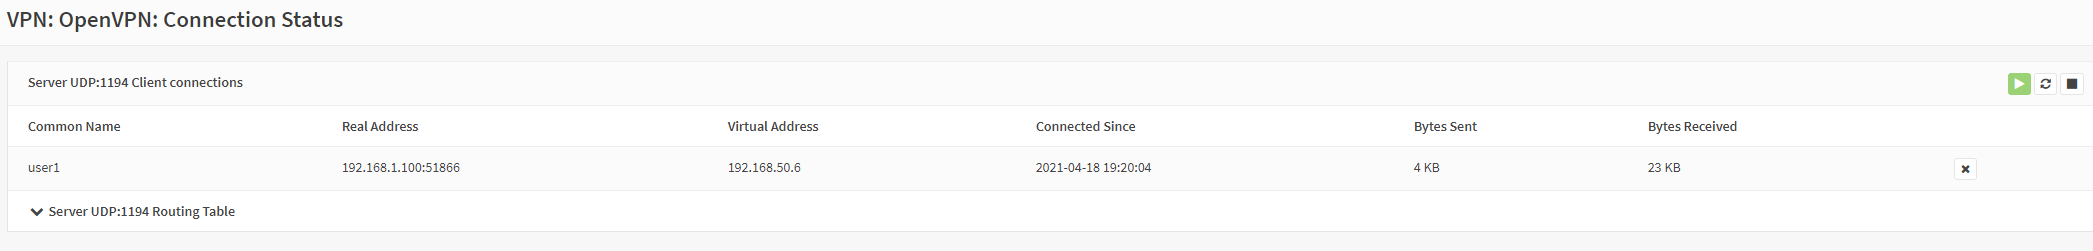
\includegraphics[width=0.8\textwidth]{Images/vpn/vpn_client_connecting_status.PNG}
    \caption{OpenVPN status on the firewall}
    \label{opnsense:vpn_openvpn_status}
\end{figure}


\quesblock{\begin{enumerate}
    \item[35.] Did you manage to connect to the firewall?
    \item[36.] What is the minimum recommended key size for RSA encryption? 
\end{enumerate}}

%---------------------------
%Questions: 1. What do you see if you are using Wireshark to capture your network traffic?
%2. 